% Figure from MATH 556 notes, section 14. Compile with the notes preamble.
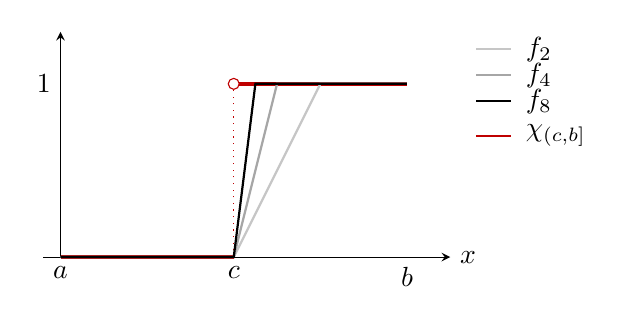
\begin{tikzpicture}[scale=2.2, >=stealth]
    \draw[->] (-0.1,0) -- (2.25,0) node[right] {$x$};
    \draw[->] (0,0) -- (0,1.3);
    \node[below] at (0,0) {$a$};
    \node[below] at (1,0) {$c$};
    \node[below] at (2,0) {$b$};
    \node[left] at (0,1) {$1$};
    \draw[very thick, red!75!black] (0,0) -- (1,0);
    \draw[very thick, red!75!black] (1,1) -- (2,1);
    \draw[dotted, red!75!black] (1,0) -- (1,1);
    \draw[red!75!black, fill=white] (1,1) circle (0.9pt);
    \foreach \n/\st in {2/gray!45, 4/gray!70, 8/black}
        \draw[thick, \st] (0,0) -- (1,0) -- ({1+1/\n},1) -- (2,1);
    \foreach \y/\st/\lab in {1.2/gray!45/{$f_2$}, 1.05/gray!70/{$f_4$}, 0.9/black/{$f_8$}, 0.7/{red!75!black}/{$\chi_{(c,b]}$}} {
        \draw[thick, \st] (2.4,\y) -- (2.6,\y);
        \node[anchor=west] at (2.63,\y) {\lab};
    }
\end{tikzpicture}
